\section{Variation of Merger Parameters and Robustness of Results}
\label{sec:c2_variation}

In our parameter space study, we focused on the effects of varying the masses of the two WDs, fixing the initial separation {\azero}, merger completion time criterion, and WD composition.  To determine how robust our results are, we ran simulations varying these assumptions.

\subsection{Changing the Composition}

\begin{figure}
\centering
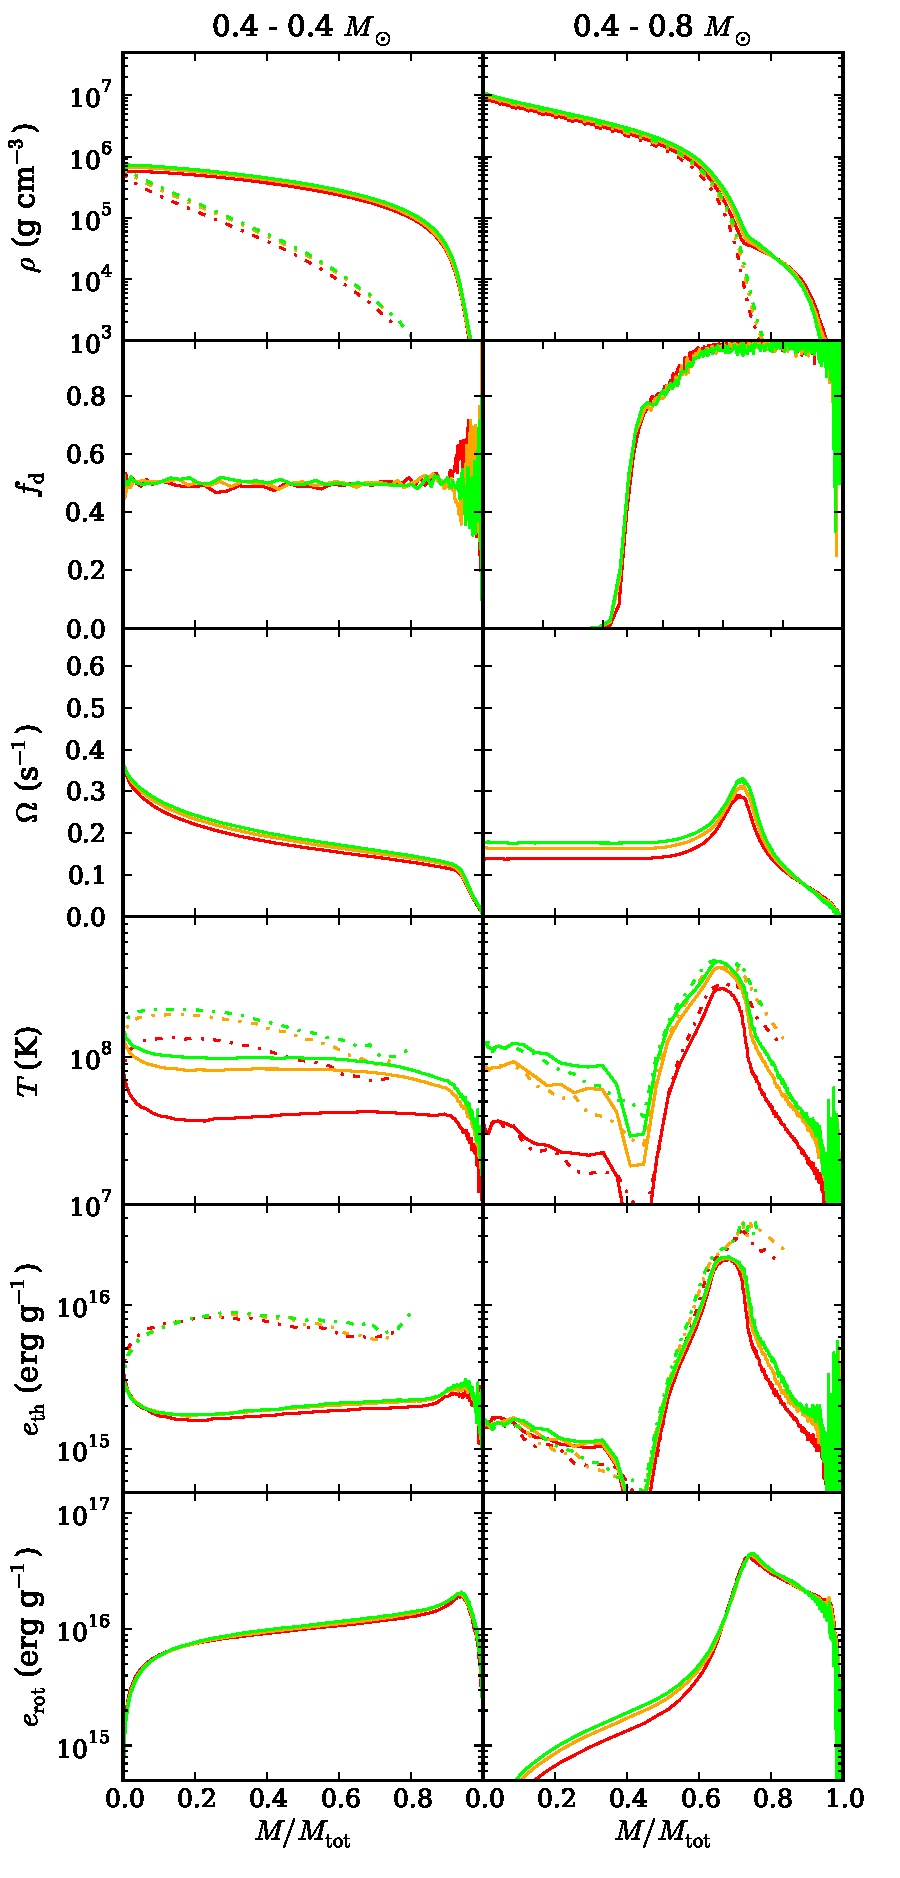
\includegraphics[angle=0,width=0.5\columnwidth]{chapter2_zhu+13/figures/compcomp.pdf}
\caption{As Fig.~\ref{fig:c2_constacc}, but for 0.4 - 0.4 {\Msun} (left) and 0.4 - 0.8 {\Msun} (right) mergers with different compositions: pure $^4$He (red), CO (orange), and pure $^{24}$Mg (lime).  Dash-dotted lines represent profiles along the rotational axis rather than the equatorial plane.}
\label{fig:c2_compcomp}
\end{figure}

Ignoring fusion, WD mergers should be insensitive to changes in composition, since the dominant electron degeneracy pressure only depends on the mean molecular weight per electron, which is close to $\mu_e\simeq2$ for all likely compositions.  To confirm this, we ran simulations assuming pure helium and pure magnesium for an equal-mass case (0.4 - 0.4\,\Msun) and an dissimilar one (0.4 - 0.8\,\Msun).  The results are shown in Figure \ref{fig:c2_compcomp}.  One sees that most quantities indeed have very similar profiles.

The set of profiles showing most variation are those of the temperature.  These have similar shape, but different normalization.  Since the thermal energy curves are very similar, it is clear that this reflects differences in heat capacity, which does depend on composition: for He composition, there are more (non-degenerate) ions than for our standard CO mixture, boosting the heat capacity (and thus lowering the temperature for given thermal energy), while for Mg composition, there are fewer, lowering the heat capacity (and increasing the temperature).  As a result, the maximum equatorial plane temperatures for the 0.4 - 0.4\,\Msun\ simulations are 0.95, 1.48 and $1.68\times10^8$ K for He, CO, and Mg, respectively, while for the 0.4 - 0.8\,\Msun\ simulations, they are 2.92, 4.05, and $4.47\times10^8\,$K.

%MHvK: with changes to above paragraph, this one became superfluous.
%A comparison of the specific thermal energy profiles hammers home this point.  Here, the thermal energy profiles, $E_{\rm therm}$ are nearly identical for the different compositions.  In particular, for the $0.4\,-\,0.8\,M_\odot$ simulations we find maximum thermal energies of $2.1\times10^{16}{\rm\,erg\,g^{-1}}$ with a deviation of about 4\%, while in the $0.4\,-\,0.4\,M_\odot$ simulations we find maximum thermal energies of $3.7\times10^15{\rm\,erg\,g^{-1}}$ with a deviation of about 10\%.  The well behaved nature of our results to variations in composition, while not realistic in nature, demonstrates that the properties of WD mergers is fairly well-understood.

The smaller differences seen for the other profiles reflect small differences in initial conditions.  All WDs are constructed assuming $T=5\times10^6\,$K throughout, which implies more thermal energy for higher heat capacity.  As a result, the relaxed He and Mg WDs are slightly larger and smaller, respectively, than the CO WD.  These slight differences in radius translate into differences in initial separation, which in turn cause small differences in the angular velocity and rotational energy curves.

\subsection{Varying the Initial Binary Separation}
\label{ssec:c2_varyingazero}

\begin{figure}
\centering
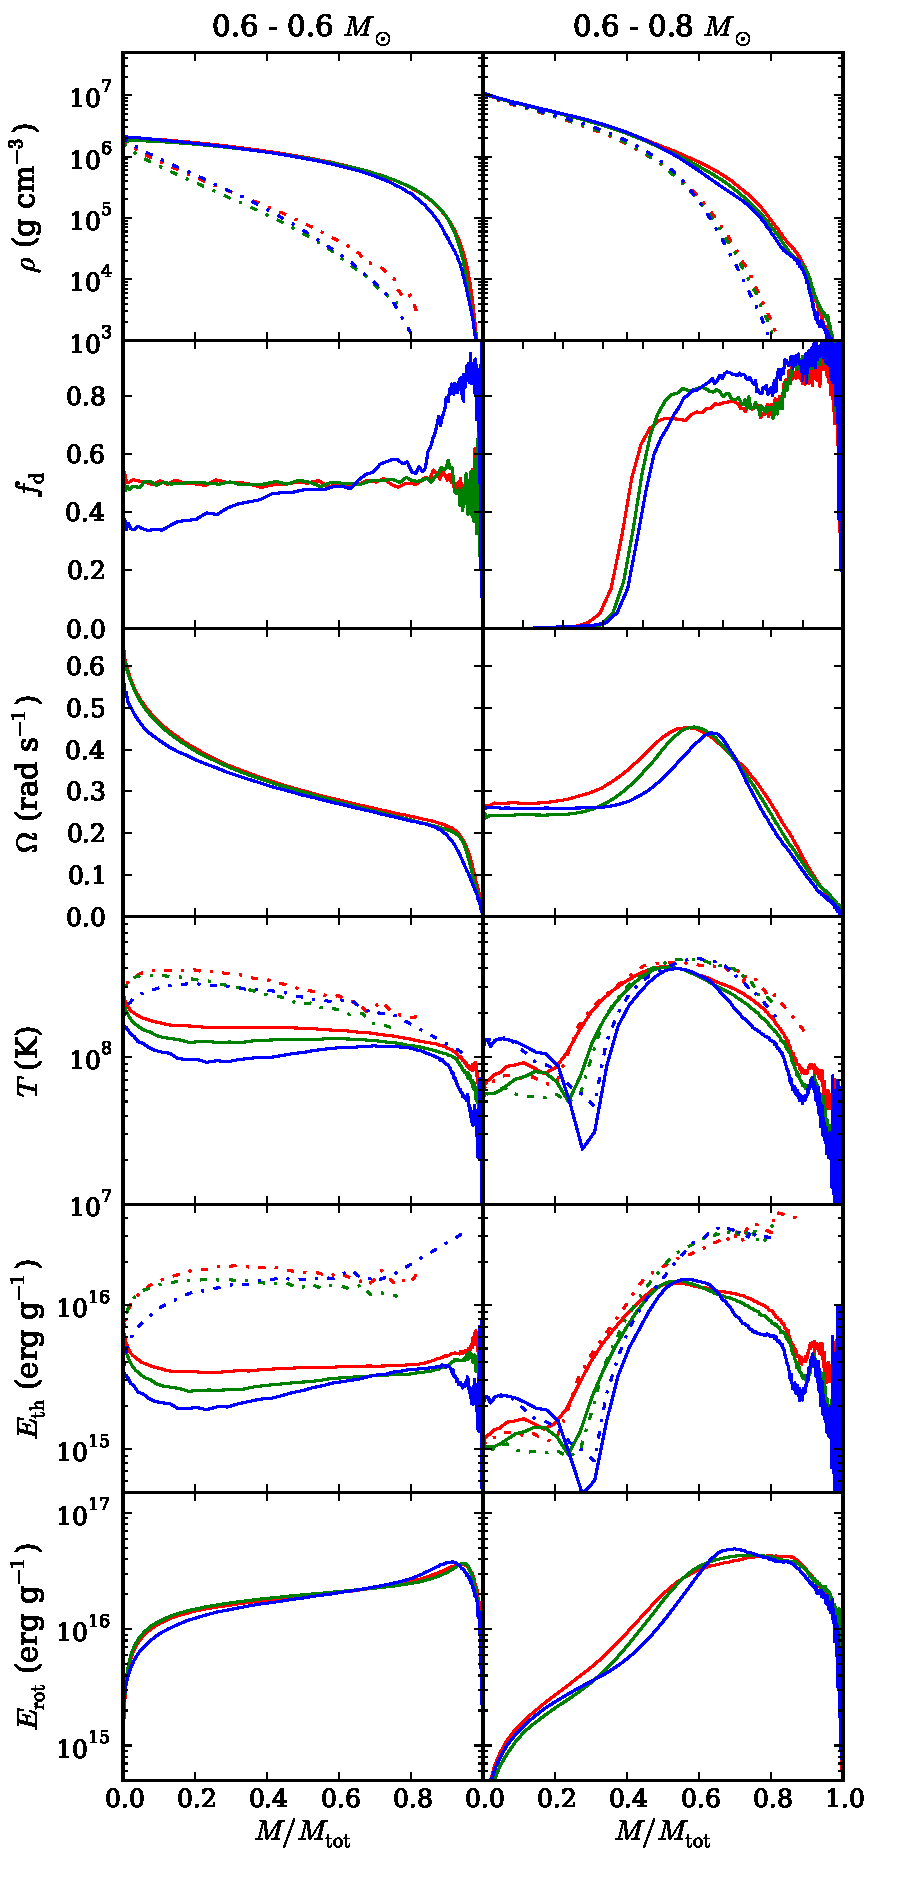
\includegraphics[angle=0,width=0.5\columnwidth]{chapter2_zhu+13/figures/distcomp.pdf}
\caption{As Fig.~\ref{fig:c2_compcomp}, but for 0.6 - 0.6 {\Msun} (left) and 0.6 - 0.8 {\Msun} (right) mergers with varying initial orbital separation: 0.9 (red), 1.0 (green), and 1.1 (blue) times the value used for the parameter space study.}
\label{fig:c2_distcomp}
\end{figure}

For our simulations, we chose an initial orbital separation {\azero} for which a co-rotating donor would fill its Roche lobe.  Since our (non-rotating) WDs are equilibrated in isolation, once the simulation starts they immediately begin to adjust to the tides and hence disrupt quickly.  Ideally, one would allow them to adjust to the binary potential and start mass transfer properly.  For non-synchronous rotation, however, this is not straightforward (see Sec.~\ref{ssec:c2_compwithothers}).  Nevertheless, we try to get a sense of the influence of this by running simulations for two cases -- 0.6 - 0.6\,\Msun\ and 0.6 - 0.8\,\Msun\ -- with \azero\ increased and decreased by 10\% (see Fig.~\ref{fig:c2_distcomp}).

Our default simulations were considered complete at 6 orbits of the initial binary.  For runs where \azero\ was changed, we used 2.5\% non-axisymmetry, and a requirement for the density to be highest at the remnant's center, as the completion criteria\footnote{The 2.5\% non-axisymmetry convergence time is 312 s (6.6 orbits) for our default 0.6 - 0.6 {\Msun} run, and 250 s (5.2 orbits) for our default 0.6 - 0.8 {\Msun} run.}.  Not surprisingly, runs with larger {\azero} needed longer to achieve these criteria: with a 10\% increase, the 0.6 - 0.8 {\Msun} merger required 861 seconds, or $\sim\!15$ orbits, to complete, while the one with a 10\% decrease required 230 s, or $\sim\!5.5$ orbits.  Similarly, the 0.6 - 0.6 {\Msun} merger with a 10\% increase in {\azero} required $\sim\!13$ orbits (725 s) to complete, compared to the 7 orbits of a 10\% decrease (283 s).  In both cases, the increase simply reflects that it takes longer for the donor to be disrupted fully if \azero\ is increased\footnote{Of course, if placed far enough, the binary does not merge.  For a 0.6 - 0.8 {\Msun} binary, no mass transfer occurred within 500 s if \azero\ was increased by 20\%.}.  For instance, for the 0.6 - 0.8 {\Msun} binary with increased separation, it took almost a dozen orbits before full disruption, while at the standard separation disruption occurred after just 1.5 orbits.  This feature is of particular interest because for mergers of synchronously rotating WDs \cite{dan+11,dan+12} and \cite{rask+12} all note almost immediate disruption of the donor when approximate initial conditions are used, and much delayed disruption for more accurate initial conditions (up to $\sim\!30$ orbits; see Sec.~\ref{ssec:c2_compwithothers}).

We find that the density profiles of the merger remnants are remarkably insensitive to varying \azero\ (\rhoc\ changing by $\lesssim2$\% for the 0.6 - 0.8 {\Msun} merger, and $\sim20$\% for the 0.6 - 0.6 {\Msun} merger), and show substantial systematic changes only in the outer regions.  The latter can be understood from the mixing and rotational profiles, where one sees that with increasing \azero, donor material is mixed less deeply into the accretor, and rotational energy is shifted outward, causing the rotational frequency to peak at lower values and larger radii.  This reflects the increase in angular momentum with increasing \azero, which creates a more rotationally supported remnant (for both our systems, a 10\% increase (decrease) in \azero\ results in a 5\% increase (decrease) in angular momentum).  In the 0.6 - 0.8\,\Msun\ merger, the decreased mixing causes the accretor to be spun up less, thus lowering the rotational energy of the core, and narrowing the thermal energy plateau.  These effects are also seen in the similar-mass case, where the center of the remnant receives less rotational support and becomes denser with increasing separation, and the mixing becomes less uniform.

Qualitatively, with increasing \azero, the properties change in a way that is similar to the changes seen with decreasing \qrho, i.e., similar to mergers with more dissimilar mass: reduced mixing, larger disks and less core rotational support, and shifts in the thermal and rotational energies toward larger radii.  The converse is also true, decreasing \azero\ has similar effects as increasing \qrho, i.e., the mergers become similar to those with more equal masses.  The changes are substantial at times: e.g. with a 10\% increase in {\azero} for the 0.6 - 0.6 {\Msun} remnant, the maximum equatorial temperature is reduced by 40\%, while the corresponding density increases by 25\% (for the rotational axis hotspots, the values are a 13\% and 30\% reduction, respectively), and the mass of the disk increases by 65\%.  Similar, though far less extreme, changes are seen for the properties of the 0.6 - 0.8 {\Msun} remnant.  All this makes {\azero} one of the parameters our mergers are most sensitive to.

%For a 10\% change in \azero, many remnant properties change substantially: e.g., {\rhoTmax} changes by $\sim\!15$\% for both mergers, while {\Tmax} decreases by 35\% for the 0.6 - 0.6\,\Msun\ merger when {\azero} is increased by 10\% (along the equatorial plane, along the rotational axis, the decrease in temperature is $\sim10$\%, and density $\sim30$\%).  For the 0.6 - 0.6 \Msun\ merger, the mass of the (very small) disk increased by 65\% for the 10\% increase in \azero, while for the 0.6 - 0.8\,\Msun\ merger, the effect was around 4\%.  Thermodynamic properties around temperature maxima are in general more robust to changes in {\azero} for the 0.6 - 0.8\,\Msun\ merger than in the 0.6 - 0.6 \Msun\ merger, while the reverse is true for core-envelope energy and angular momentum.  {\bf CZ: does this paragraph have any use??}

%CZ: This is not true (and you can tell from the figure that the equal mass and unequal mass mergers both change substantially)!!!
%In general, the similar-mass merger changed more drastically than the unequal mass one: for the former, only the central scale height and global energy balance did not change, while for the latter, the maximum temperature, maximum angular velocity, their enclosed masses, and generally most properties of the remnant core changed by less than 10\%.  Hence, if more accurate initial conditions would substantially change the effective initial separation, we expect nearly equal mass mergers to be affected more than unequal mass ones.

%change on average by $\sim20$\% \emph{THIS IS AN AVERAGE OVER ALL REMNANT PROPERTIES, NOT JUST ONES WE CARE ABOUT}, roughly the same as, with the notable exceptions of central temperature and $\Omega$, the location of maximum $\Omega$, and energies in the disk, all of which change by $\sim20$\%.  A few properties, such as central density, pressure and entropy, scale heights, {\Tmax}, {\MencTmax}, {\Omegamax}, disk radius and remnant energies, do not change by more than $\sim15$\% even if {\azero}

%This does not directly translate to an increased number of orbits completed by the binary before total disruption of the donor, but increasing the separation even further does produce an extended survival time for the binary before coalescence, the time when the donor is totally disrupted.  Preliminary tests with suggest that past $\sim1.7a_\mathrm{0,Egg}$, the binary survives for dozens of orbits, during which a small trickle of mass transfers from the donor to the accretor.  This feature is of particular interest because \cite{dan+11}, \cite{dan+12} and \cite{rask+12} all note almost immediate coalescence for their co-rotating WD mergers when approximate initial conditions are used, and much longer (\citet{dan+11,dan+12} give up to $\sim30$ orbits for some systems) times when more accurate initial conditions are substituted.  This is discussed further in Sec. \ref{ssec:c2_compwithothers}.

%The extra time is due to the extra several orbits the two WDs complete before the 0.6 {\Msun} WD is fully disrupted.  \cite{dan+11}, \cite{dan+12} and \cite{rask+12} all note an artificially short coalescence time for their synchronized systems when approximate initial conditions are used, and suggest that a long (\citet{dan+11,dan+12} give up to $\sim30$ for some systems) coalescence time is the hallmark result of a simulation proper initial conditions.  Since placing individually relax WDs in a binary where one WD is overflowing its Roche lobe is to some degree unphysical, placing the WDs further apart should be more realistic, and therefore this result may hint at a similar effect for unsynchronized systems.

%the rotation and surface density curves and how much of the donor and accretor mass make up the disk and core all vary significantly with separation distance.  Near the Eggleton separation and above it, these values vary much more slowly: for a 10\% increase or decrease in {\azero}, properties of the remnant (listed in Tables \ref{table1} - \ref{table6}) all change by less than 10\% except for the central temperature ($\sim15$\%), moments of inertia ($\sim20$\%), rotational energy of the remnant ($\sim15$\%), and density, temperature, average angular velocity and rotational of the disk (all $\sim20$\%).  Using separations much larger than given in Eqn. \ref{eggletonrad} (by more than about 25\%) changes the number of orbits the accretor survives before it is disrupted, and affects significantly the central temperature ($\sim50$\%), central angular velocity ($\sim20$\%), density of the disk ($\sim25$\%), and total moment of inertia ($\sim$60\%) of the merger remnant (all to be expected from adding more angular momentum into the system), while leaving the general curve shapes of the remnant roughly the same.  We therefore feel using Eqn. \ref{eggletonrad} is sensible.

%Table \ref{tab:sync_async} show a few of the global quantities of this merger.

%\begin{deluxetable}{lcccc}%\tabletypesize{\tiny}
%\tablecaption{Synchronous vs asynchronous endpoints\label{tab:sync_async}}
%\tablehead{
%	\colhead{Property} &
%	\colhead{0.6-0.6a} &
%	\colhead{0.6-0.6s} &
%	\colhead{0.8-0.6a} &
%	\colhead{0.8-0.6s}
%}
%\startdata
%$L_{\rm tot}$ ($\times 10^{50}$) & 3.53 & 3.94 & 4.09 & 4.50 \\
%$L_{\rm rem}$ ($\times 10^{50}$) & 2.68 & 2.19 & 1.30 & 1.37 \\
%$M_{\rm rem}$ & 1.12 & 1.02 & 1.08 & 1.05 \\
%$M_{\rm disk}$ & 0.084 & 0.182 & 0.326 & 0.351 \\
%$M(0.5 M_{\rm d})$ & 0.597 & 0.577 & 1.02 & 1.03 \\
%$T_{\rm max}$ ($\times 10^8$ K) & 3.44 & 2.35 & 5.00 & 3.76 \\
%$M_{\rm enc}(T_{\rm max})$ & 0.001 & 0.000 & 0.683 & 0.789 \\
%$M_{\rm enc}(0.5 E_{\rm therm})$ & 0.436 & 0.496 & 0.824 & 0.836 \\
%$\Omega_{\rm max}$ & 0.804 & 0.593 & 0.502 & 0.466 \\
%$M_{\rm enc}(\Omega_{\rm max})$ & 0.000 & 0.000 & 0.887 & 0.872 \\
%$M_{\rm enc}(0.5 E_{\rm rot})$ & 0.764 & 0.836 & 1.09 & 1.06 \\
%$E_{\rm rot,rem}$ ($\times 10^{49}$ ergs) & 4.15 & 3.35 & 3.08 & 3.00
%\enddata
%\end{deluxetable}

\subsection{Synchronization}
\label{ssec:c2_synchronization}

\begin{figure}
\centering
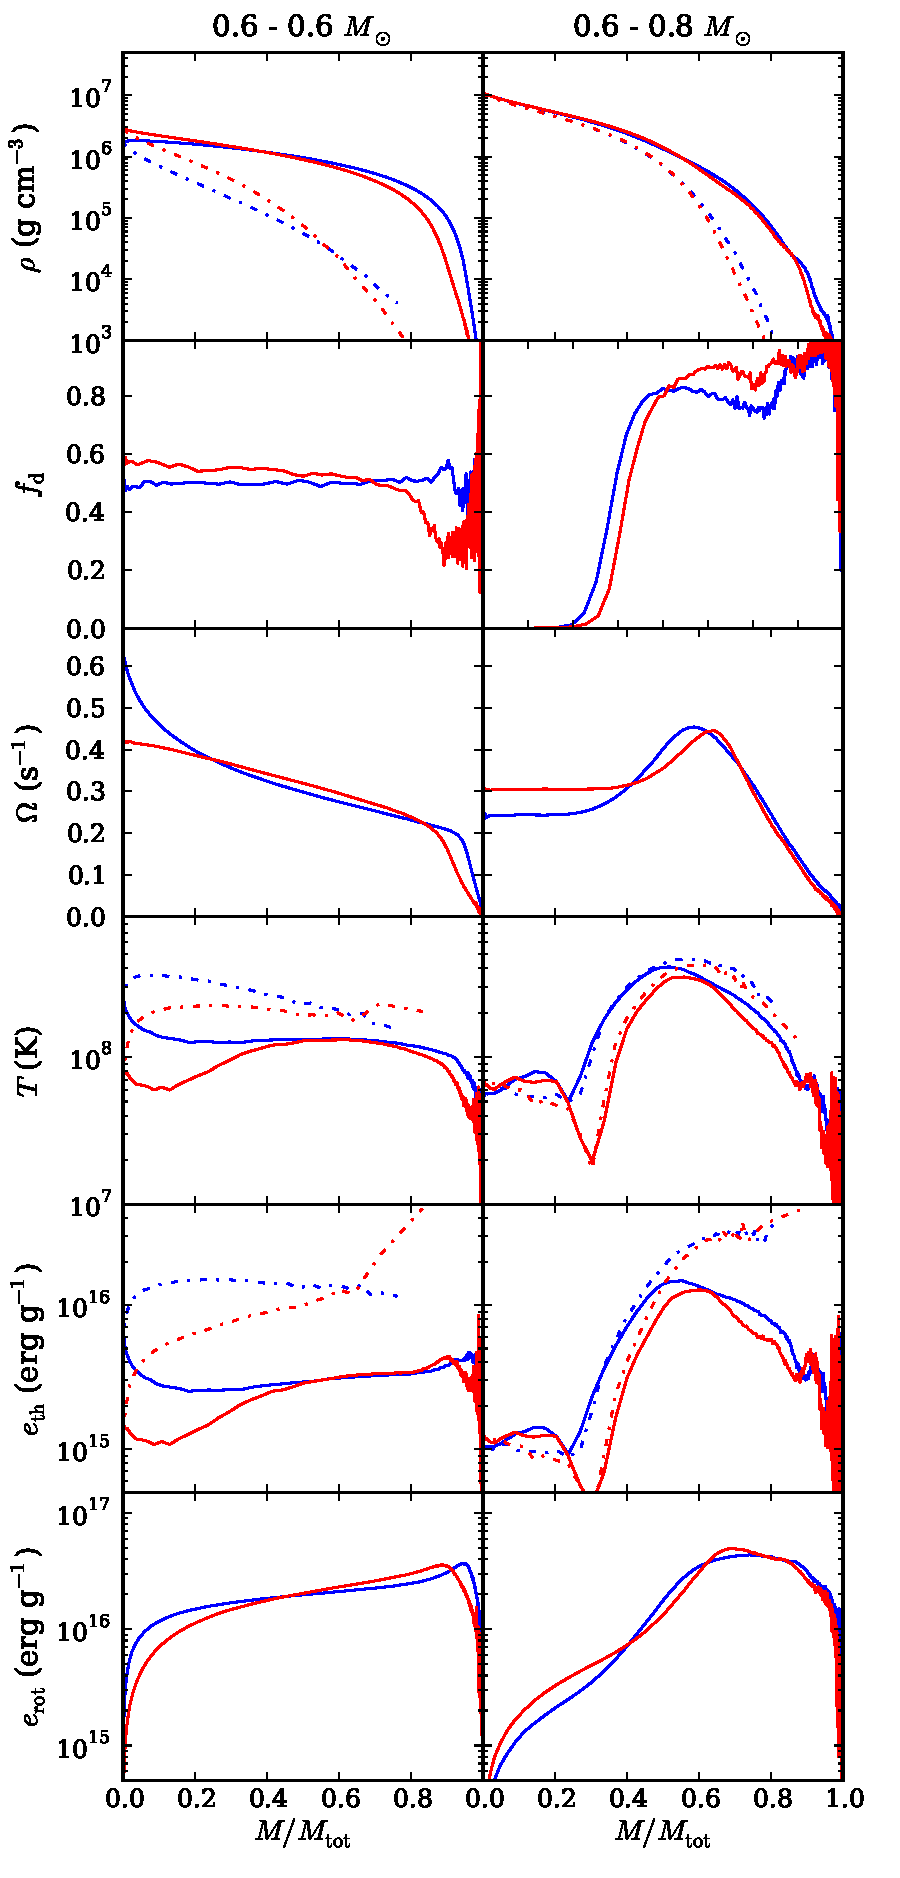
\includegraphics[angle=0,width=0.5\columnwidth]{chapter2_zhu+13/figures/synchcomp.pdf}
\caption{As Fig.~\ref{fig:c2_compcomp}, but for 0.6 - 0.6 {\Msun} (left) and 0.6 - 0.8 {\Msun} (right) mergers, comparing our default, irrotational case (blue) with that assuming synchronous rotation (red).}
\label{fig:c2_synchcomp}
\end{figure}

In our simulations, the WDs have zero spin, i.e., we assume that tidal dissipation is too weak to synchronize their rotation.  Whether or not this is correct is currently unknown, but to see what the effect could be, we ran simulations assuming synchronized rotation for 0.6 - 0.6\,\Msun\ and 0.6 - 0.8\,\Msun\ binaries (see Fig.~\ref{fig:synchcomp}).  We used approximate initial conditions for these systems, identical to those of Sec. \ref{ssec:c2_initcond} except that the stars rotate at the orbital angular frequency.

As in Sec.~\ref{ssec:c2_varyingazero}, our unsynchronized runs are from our parameter space study, and use 6 orbits as their completion criterion, while our synchronized runs use 2.5\% non-axisymmetry, and a requirement for the density to be highest at the remnant's center.  Completion occurred at 407 s ($\sim$8.5 orbits) for the synchronized 0.6 - 0.6 {\Msun} simulation, and 314 s ($\sim$6.5) orbits for the synchronized 0.6 - 0.8 {\Msun}.

The asynchronous and synchronous mergers differ mostly in the amount of heating and spin-up.  This has two causes.  First, for the synchronized binary, the total amount of angular momentum is about 10\% larger, and high angular momentum material has more difficulty penetrating the accretor, as is evident in the 0.6 - 0.8 {\Msun} mixing profile (because of the larger amount of angular momentum, the mergers also take about 1.5 orbits longer to achieve 2.5\% non-axisymmetry).  Second, in a synchronized binary, the donor and accretor have much less differential rotation with respect to each other, leading to much less spin-up and heating.

Both effects are largest for the equal-mass case.  In particular, in a synchronized, equal-mass binary contact can occur without any friction, while in an unsynchronized one it involves shocks at the full orbital velocity.  In consequence, for the synchronized case, rotational support is weaker in the center and stronger in the outskirts, causing the central density of our 0.6 - 0.6 {\Msun} remnant to increase by $\sim70$\% and the disk mass to increase by a factor of 2.  Furthermore, while for the non-synchronized case, the maximum temperature along the equatorial plane was found in the center, for the synchronized case it is found in the outskirts, and is more than a factor two lower ($1.3\times10^8\,$K instead of $2.9\times10^8\,$K).  The hotspots on the rotational axis also have much reduced temperature, $2.3\times 10^8$\,K instead of $3.6 \times 10^8$\,K.  
%This overall lowering of temperature, and change in the location of equatorial maximum temperature, are due to the initial accretion streams and dense torus produced during equal mass mergers experiencing much less heating in the synchronous case.

For the dissimilar-mass merger, the effects of synchronization are less dramatic: the accretor still spins up substantially, and rotational and thermal energy are deposited in roughly the same way.  The main difference is that the synchronized case has slightly less mixing, causing a drop in total thermal energy and maximum temperature (from $4.1\times10^8$ K to $3.5\times10^8$ K on the equatorial plane, and from $4.6\times10^8$ K to $4.3\times10^8$ K on the rotational axis).

%The main difference between the asynchronous and synchronous cases is the total amount of angular momentum in the system: $L_{\rm tot}$ is about 10\% larger in the synchronous case compared to the asynchronous case.  This does not necessarily translate to greater angular momentum in the remnant, $L_{\rm rem}$, because high angular momentum material has difficult accreting.  This is seen in the masses of the remnants where the masses of the synchronous cases is smaller than that of the asynchronous cases, while the masses of the disk is larger (at least in the 0.6-0.6 case).  The reduced angular momentum of the remnants translates into a lower value of $\Omega_{\rm max}$ and $E_{\rm rot,rem}$ in the synchronous case, while the mass coordinate of $\Omega_{\rm max}$ seems unaffected.  The smaller masses of the remnants also appears to translate to a lowering of the maximum temperature in the synchronous cases and in moving its mass coordinate in the case of the 0.8-0.6 merger.

\subsection{Running the Simulation Longer}
\label{ssec:c2_runninglonger}

\begin{figure}
\centering
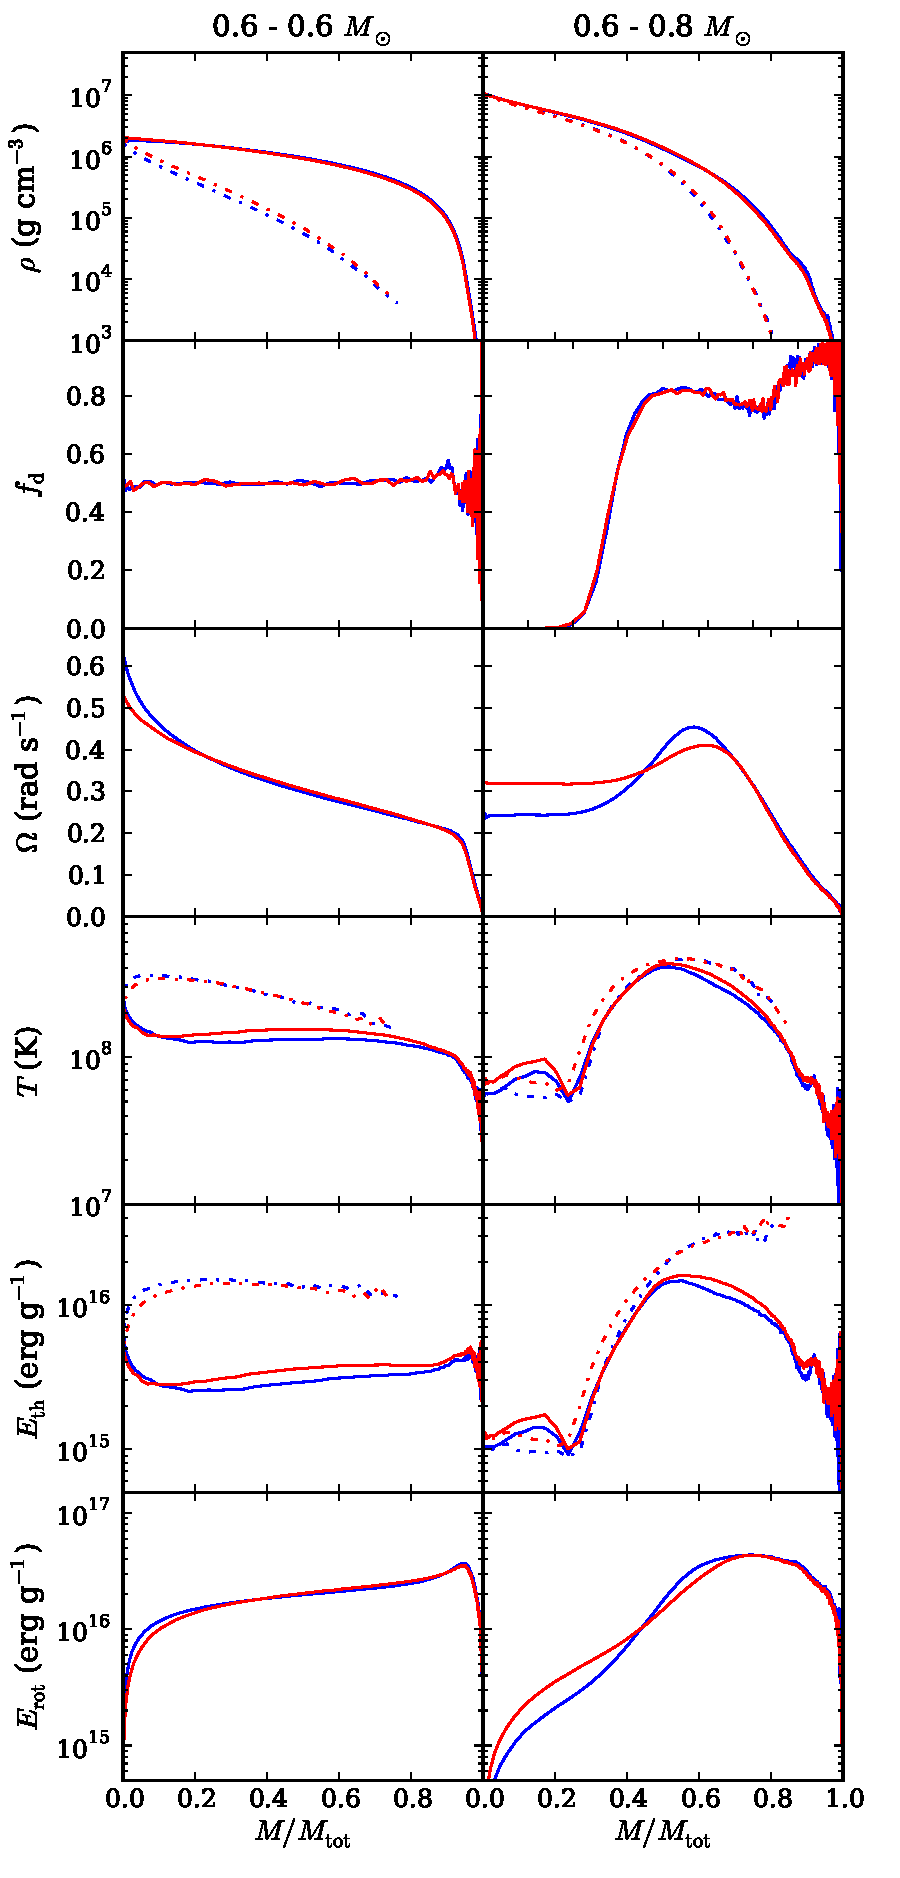
\includegraphics[angle=0,width=0.5\columnwidth]{chapter2_zhu+13/figures/timecomp.pdf}
\caption{As Fig.~\ref{fig:c2_compcomp}, but for 0.6 - 0.6 {\Msun} (left) and 0.6 - 0.8 {\Msun} (right) mergers, comparing properties for our default simulation time of 6 initial orbital periods (blue) with those obtained after 8 orbital periods (red).}
\label{fig:c2_timecomp}
\end{figure}

We considered our mergers completed after 6 orbits, since in that time they on average had reached our convergence criterion of 2.5\% non-axisymmetry (see Sec.~\ref{ssec:mergercomplete}).  To test the robustness of our results, we also determined properties attained after 8 orbits.  In Fig.~\ref{fig:c2_timecomp}, we compare the 6 and 8 orbit results for 0.6 - 0.6\,\Msun\ and 0.6 - 0.8\,\Msun\ binaries.

We find our mergers show little evolution between 6 and 8 orbits, with the largest changes seen for the angular velocity profiles.  For the 0.6 - 0.8 {\Msun} merger, the rigidly rotating core sped up and the off-center peak decreased in height and moved out, while for the 0.6 - 0.6 {\Msun} merger, the center spun down and the rotational profile became flatter.  In the dissimilar-mass merger, \Tmax\ and \rhoTmax\ changed by $\lesssim\!5$\% and the density and temperature structures nearly overlap, while in the equal-mass merger \Tmax\ and \rhoTmax\ changed by $\sim\!20$\% ($2.9$ to $2.3\times10^8\,$K and $1.7$ to $2.0\times10^6\,\gcc$), reflecting an increase in central density and a shifting of the temperature profile, with temperature decreasing in the center but increasing elsewhere.  The evolution of all properties is consistent with viscous evolution -- expected to follow the merger proper -- with the core driven into rigid rotation, and angular momentum transferred outward to the disk.  In the dissimilar-mass merger, the net effect is spin-up of the core and spin-down of the envelope, while in the equal-mass case it is the reverse.  Of course, in the process, rotational energy is turned into thermal energy, heating the remnants.

One curious aspect for equal-mass mergers is the evolution of the off-center hot spots (Fig.~\ref{fig:c2_mergersampling2}).  Over time, these broaden parallel to the equatorial plane, yet become narrower along the rotational axis.  As a result, the hourglass shape is lost, and the center of the remnant stops being one of the hottest point in the system.  After 8 orbits, the system resembles more closely what we find for typical similar-mass mergers, which have more pancake-shaped hot spots flanking a colder, denser region on the equatorial plane.

%Comparing more broadly the 6 and 8-orbit results, we find changes at the $\lesssim\!5$\% level.  Exceptions include the central temperature, which changes by 20\% (for unequal masses this is due to a combination of spurious heating and heating due to spin-up, while for equal mass mergers the reason is detailed above), \Tmax\ by 7\%, \rhoTmax\ by 9\%, and \Omegamax\ by 9\%.  The density and enclosed mass of the hottest point along the $z$-axis can also shift substantially, partly due to the evolution of the off-center hotspot in equal mass mergers, and partly due to noise in the tenuous envelope.  With viscous evolution towards rigid rotation, we also see changes of up to 10\% in the core-envelope and disk rotational energy and angular momentum.

%When comparing the entire set of merger remants found using 2.5\% non-axisymmetry to those found using 1\%, the central density has increased $\sim$15\% for equal mass mergers (negligibly for unequal mass mergers), while the central temperature has increased $\sim$9\% for unequal mass mergers (though this may be due to spurious heating; see Sec. \ref{ssec:spheat}).  The maximum temperature has not changed significantly, but {\rhoTmax} has increased by $\sim$13\% for all mergers.  The disk has decreased by $\sim$5\% for unequal mass mergers (more than $\sim$10\% for highly unequal mass mergers), and increased by $\sim3$\% for equal mass mergers.  For unequal mass mergers the central $\Omega$ has increased by an average of $\sim$16\% with a corresponding drop in {\Omegamax} by $\sim$4\%, while for equal mass mergers the central $\Omega$ has dropped by $\sim$10\%.  All these trends are consistent with those seen in Fig. \ref{fig:timecomp}, indicating the figure's curves as being generalizable to all equal and non-equal mass mergers.  \textbf{CUT THIS PARAGRAPH?}

Comparing more broadly the 6 and 8-orbit results, we find changes at the $\sim\!5$\% level.  The trends presented in Sec.~\ref{ssec:c2_mergertrends} continue to hold to within $\sim\!10$\% except for \hxy\ (which becomes $\hxy/h_{\rm a} = 0.98 + 0.74q_\rho^2~(\pm0.07)$), the fraction of disk energy in degeneracy energy ($E_\mathrm{deg,disk}/E_\mathrm{I,disk} = 0.07~(\pm0.02)$), mass enclosed within the radius of maximum temperature ($\MencTmax/\Ma = 1-0.21q_\rho~(\pm 0.01)$), maximum rotational frequency ($\Omegamax/\Omegaorb = 3.4~(\pm0.5)$) and the widths of the regions in which thermal and rotational energy are deposited ($\MEthermthick/\Ma = 0.13 + 0.87q_\rho ~(\pm0.03)$; $\MErotthick/\Ma = 0.15 + 0.70q_\rho ~(\pm0.02)$).  Changes to these trends are consistent with the viscous evolution described above: the remnant is beginning to spin down, lose its rotational support, and energy is being redistributed.

\subsection{Viscosity Prescription}
\label{ssec:c2_viscprescrip}

The addition of artificial viscosity is required in SPH to accurately capture shocks, but no consensus exists on how best to implement it.  We ran two additional simulations of a 0.6 - 0.8\,\Msun\ merger to check the robustness of our results with respect to changes in the viscosity, one with small and one with large artificial viscosity (fixed $(\alpha,\beta)=(0.05,0.1)$ and $(1,2)$, respectively).  As before, these additional runs use 2.5\% non-axisymmetry and a requirement for the density to be highest at the remnant's center as their completion criteria, and the low viscosity run completed at 198 s while the high completed at 242 s.  Here, we expect that low values of $\alpha$ will lead to large particle noise and inaccurate shock capturing, while high values result in large viscous heating and rapid loss of differential rotation.  Our results confirm this (Fig.~\ref{fig:c2_viscnumcomp}): the simulation with low artificial viscosity leads to a remnant with stronger differential rotation, with the disk carrying 34\% more rotational energy (and the remnant 33\% less) than in the standard variable $\alpha$ simulation.  Lower viscosity also leads to greater mixing of donor and accretor material, reflecting the stronger diffusion associated with the larger particle noise inherent to low viscosity.

Aside from the mixing and spin-up, the results for the three different viscosity prescriptions do not differ greatly.  While one might have expected greater dissipation of rotational into thermal energy for higher viscosity, the maximum temperatures and rotation rates vary by $\lesssim\!10$\%, and the thermal and rotational profiles are quite similar.  The density profiles are virtually identical except near the outer parts, where the low viscosity simulation leaves matter with greater rotational support.  

%CZ: This is wrong, according to James - his e-mails indicate he does not think spurious heating goes up with lower viscosity.  "The largest and initially most curious difference between the three simulations is that of central temperature, where for high viscosity we find a low central temperature and for low viscosity a high one.  This reflects the changes in spurious heating due to particle noise, which we discuss next."

%MHvK: keeping this sentence about equal-mass mergers is an invitation for a referee to ask why we do not test that...
%Both the density and temperature curves, however, might change more for equal mass mergers, since mixing of the entire remnant is a more important contributor to the final remnant structure in those cases.

%To determine how much our viscosity prescription can affect the outcome of our merger, we ran a 0.6 - 0.8 {\Msun} merger with the viscosity artificially low ($\alpha\,=\,0.05$, $\beta\,=\,0.1$) and artificially high ($\alpha\,=\,1.0$, $\beta\,=\,2.0$).  The former should be unable to properly capture any shocks that arise during the initial merger, while the latter will produce unphysically large viscous heating and reduction of differential rotation following the merger.  The results reflect this (Fig. \ref{fig:viscnumcomp}): mixing in the low-viscosity run is more thorough than in the high-viscosity one (where friction stops the donor from penetrating into the accretor).  The spin-up of the remnant core is much greater in the high-viscosity run, and the temperature peak is also higher and more narrow (due to lack of donor penetration).  Since most of the support of the remnant against gravity is due to degeneracy pressure, the density curves do not differ significantly.  Curiously, while most of the variable $\alpha$ curves resemble their low viscosity counterparts, the rotation and rotational energy curves more closely match the high viscosity ones.  This is perhaps because the angular velocity curve structure is set during the first few seconds of merger, just after the donor is disrupted, or perhaps during the latter stages of the merger $\alpha$ is still high in the $\Omega$ peak.  \textbf{I'M MAKING MOVIES TO SEE WHICH IS TRUE.}

%Many of the merger remnant properties change by more than 20\% between the different viscosity runs, including the number of orbits required to complete merger ($\sim25$\%), the central and maximum temperature ($\sim30$\% for {\Tc} and $\sim25$\% for {\Tmax}), {\MencTmax} ($\sim25$\%), and the disk energies ($\sim20$\% on average).  Density values unassociated with {\Tmax} and {\Omegamax} remain largely unchanged (ex. {\rhoc} changes by 2\% from variable $\alpha$ for both high and low viscosity).  Comparative runs for our entire parameter space have not been completed, so it is not certain if the remnant trends will still scale as they do in Sec. \ref{ssec:mergertrends}.

\begin{figure}
\centering
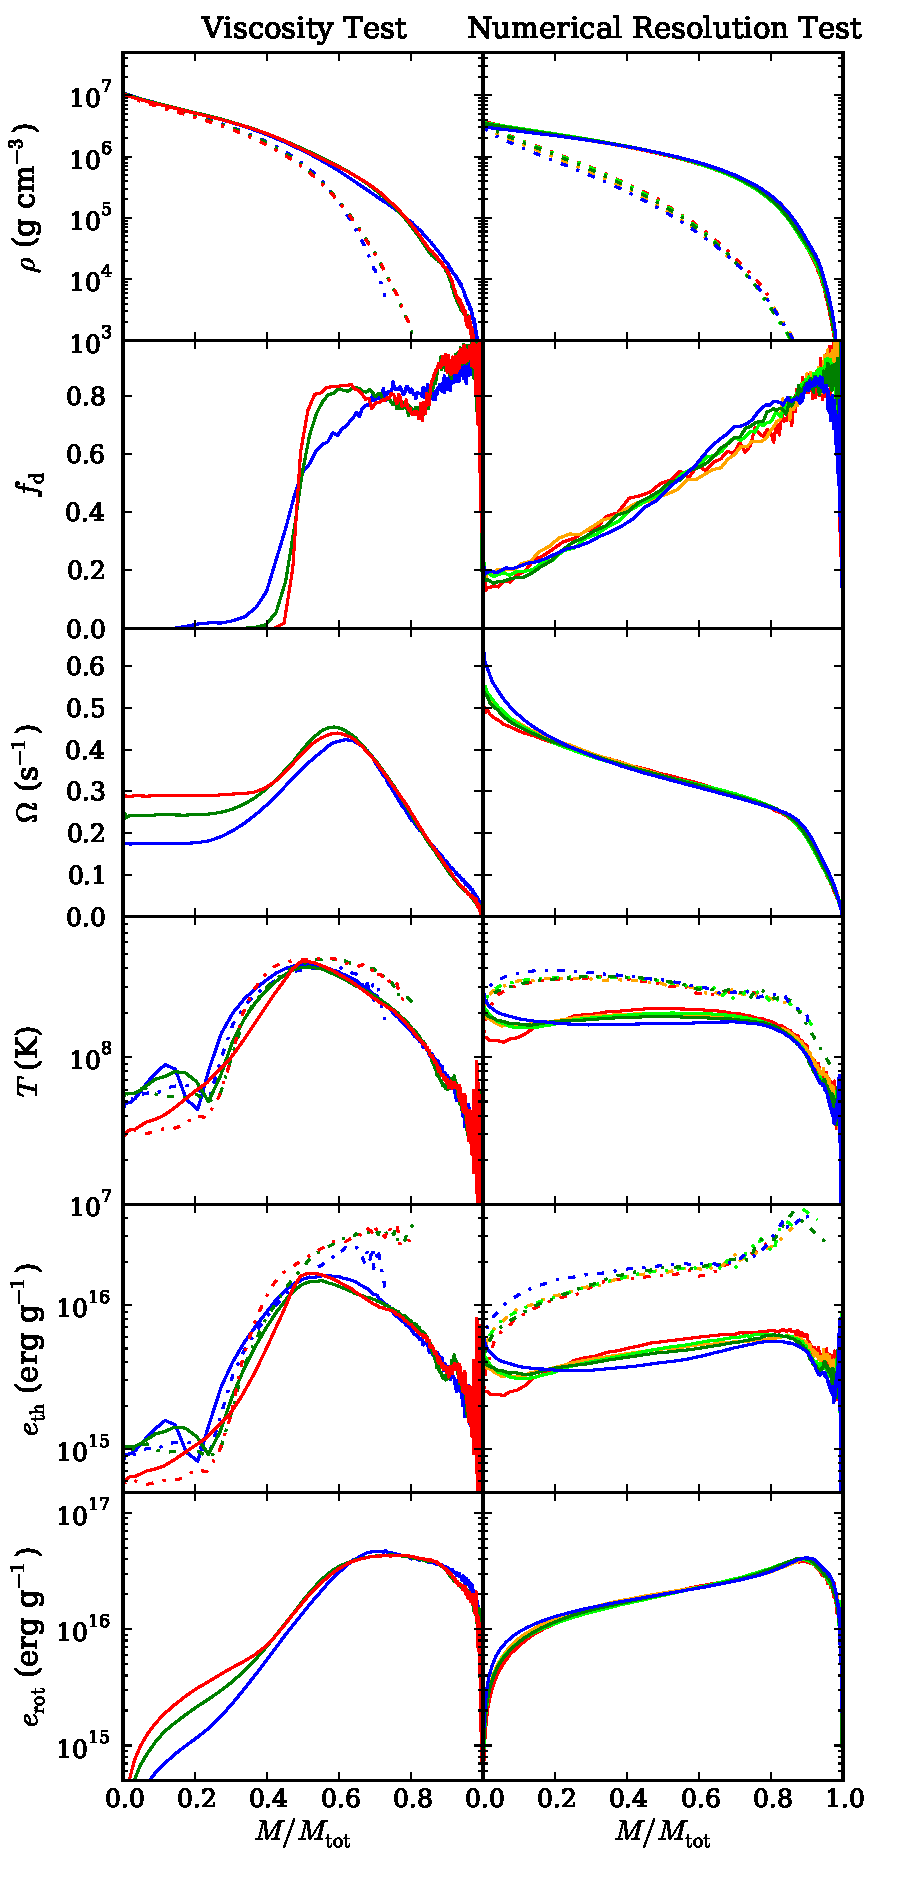
\includegraphics[angle=0,width=0.5\columnwidth]{chapter2_zhu+13/figures/viscnumcomp.pdf}
\caption{As Fig.~\ref{fig:c2_compcomp}, but comparing simulations of a 0.6 - 0.8\,\Msun\ merger with different viscosity prescriptions (left) and simulations of a 0.625 - 0.65\,\Msun\ merger with different numbers of particles (right).  For the viscosity, we compare fixed low viscosity ($\alpha=0.05$, $\beta=0.1$; blue), standard variable viscosity (green), and fixed high viscosity ($\alpha=1.0$, $\beta=2.0$; red).  For particle numbers, we show simulations at one quarter (red), half (orange), and double (blue) the default number of particles, as well as the default simulation (lime) and a rerun of the default simulation (green) to determine the effect of order-of-execution differences, round-off errors and other such numerical effects.}
\label{fig:c2_viscnumcomp}
\end{figure}

\subsection{Spurious Heating}
\label{ssec:c2_spheat}

As discussed in Sec.~\ref{ssec:c2_sphcode} and throughout Sec.~\ref{sec:c2_results}, noise combined with a pressure floor in the equation of state lead to small increases in internal energy.  While this energy has a negligible effect on most remnant properties, in the most degenerate regions of the remnant it can cause significant temperature increases.  Here, we discuss the extent to which spurious heating affects our results.

As a comparison for the spurious heating seen in some of the simulations, we relaxed a 0.8\,\Msun\ isolated white dwarf for $489\,$s longer than the standard 81\,s we used for relaxing single stars.  While the total energy of the WD (potential, degeneracy and thermal energy combined) increased by $\sim\!1$\% of the original total energy over the additional period of time, the change in thermal energy was enough to raise the central WD temperature from $1.2\times 10^7$ K (increased from $5\times 10^6$ K due to particle noise) to $1.2\times 10^8\,$K.  In Fig.~\ref{fig:c2_heating}, we compare the thermal energy profile of this isolated 0.8 {\Msun} WD with those of a 0.4 - 0.8\,\Msun\ and a 0.7 - 0.8\,\Msun\ merger, with the times for the isolated WD taken at 489 and 224\,s (the mergers' respective completion times) longer than the standard 81\,s.  The total thermal energy generated in the WD at an additional 489\,s is $\sim$10\% of the thermal energy generated in a 0.4 - 0.8\,\Msun\ merger.\footnote{A $\sim$10\% increase in thermal energy corresponds to $\sim\!1$\% increase in the overall energy of the 0.4 - 0.8\,\Msun\ remnant, somewhat larger than the typical $\sim\!0.3$\% level at which Gasoline conserves total energy in our simulations.  We find that similar-mass simulations tend to lose total energy at the 0.05\% level, while some of the low {\qrho} mergers gain more than 1\% in total energy due to spurious heating.}  Indeed, given how well the specific thermal energy profiles match in the interior, it is clear that spurious heating dominates there.  

Spurious heating is much less important for the 0.7 - 0.8\,\Msun\ merger, since its core has mixed to much greater extent and less time was needed for the merger to complete.  The total thermal energy generated in the isolated WD at 224\,s is only $\sim\!3$\% of the thermal energy generated during merger, and even at the very center spurious heating contributes $\sim\!35$\% (rather than nearly all) of the thermal energy.  As a result, the central temperature of the merger, $1.4 \times 10^8\,$K, is substantially higher than that of the isolated WD, $7.8 \times 10^7\,$K.  It is important to note this comparison overestimates spurious heating, since the isolated WD will have had many more particles that dip below the Fermi energy than the much hotter merger remnant core. 

%MHvK: bit unclear about point of this, so shortened
%We note that post merger heating of remnant cores is at least partly also due to spin-up of the core, and that in equal mass mergers there is little in terms of thermal evolution of the core to suggest spurious heating is actually occurring.  We therefore do not know for certain if spurious heating results from a lone, inert WD can directly be applied to our merger remnants.  Nevertheless, when the center of a merger remnant has not been heated by the merger to temperatures above $10^8$ K, we believe spurious heating provides a substantial contribution to the total energy of the core.  This renders core temperature would be higher than expected for these systems.  The effect should not be significant for high density material with $T\gtrsim3\times10^8$ K where spurious heating is small compared to the thermal energy, and for low-density ($\rho \lesssim10^5$ {\gcc}) material where the material is non-degenerate.    

Overall, we conclude that spurious heating is present, but is recognized fairly easily and does not influence our conclusions.  In particular, its effects on remnants should be small in both high-density regions with $T\gtrsim3\times10^8$\,K and in lower-density $\lesssim\!10^6\,\gcc$ regions.  Other simulations may suffer from spurious heating as well.  In this respect, it is intriguing that our equatorial temperature curves for a 0.6 - 0.8\,\Msun\ merger are a good match those of \citetalias{loreig09}, even in the center (Fig.~\ref{fig:c2_compwithloreig}; Sec.~\ref{ssec:c2_compwithloreig}).

%The spurious heating may be minimized by an appropriate choice of the viscosity prescription.  For instance, a larger viscosity would reduce particle noise, which in turn would reduce spurious heating.  However, a large viscosity would also increase dissipation of differential rotation.  Other simulations may suffer from spurious heating as well.  In this respect, it is intriguing that our equatorial temperature curves for a 0.6 - 0.8\,\Msun\ merger are a good match those of \citetalias{loreig09}, even in the center (Fig.~\ref{fig:compwithloreig}; Sec.~\ref{ssec:compwithloreig}).

\begin{figure}
\centering
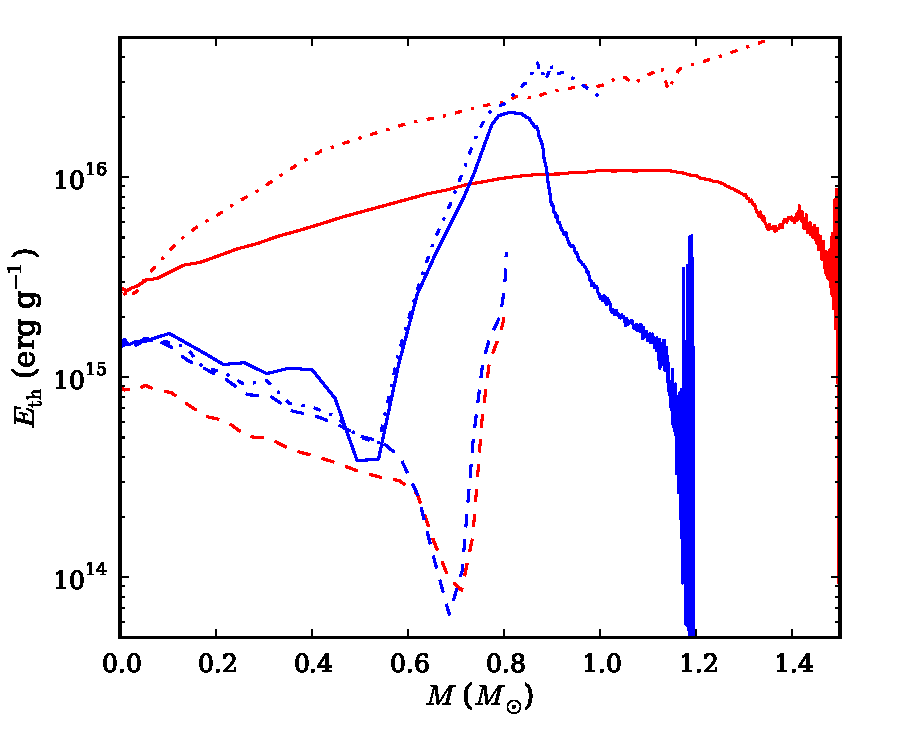
\includegraphics[angle=0,width=0.5\columnwidth]{chapter2_zhu+13/figures/heatingTEC.pdf}
\caption{Specific thermal energy as a function of enclosed mass for a 0.4 - 0.8 {\Msun} (blue) and a 0.7 - 0.8 {\Msun} merger (red), shown both along the equatorial plane (solid curves) and along the rotational axis (dot-dashed).  Also shown are the (spherical) profiles found for an isolated 0.8\,\Msun\ white dwarf (dashed) simulated using the same parameters, and for the same completion times (six initial orbital periods, equivalent to 489 s and 224 s).  Spurious heating is estimated to be responsible for nearly all the thermal energy in the core of the 0.4 - 0.8\,\Msun\ remnant, and for about one third in the core of the 0.7 - 0.8\,\Msun\ remnant.  It is not important in regions heated by interaction.  (The ``hook'' in the outer layers of the white dwarf profile reflects the high initial temperature chosen; in a merger, this is erased by the interaction.)}
\label{fig:c2_heating}
\end{figure}

\subsection{Resolution}
\label{ssec:c2_restest}

%\begin{figure}
%\centering
%\includegraphics[angle=0,width=0.35\columnwidth]{numcomp.pdf}
%\caption{Comparison of 0.625 - 0.65 {\Msun} mergers performed at different numerical resolutions.  Red indicates 63,736 (1 particle = $4\times10^{28}$ g), orange 127,525 ($2\times10^{28}$ g), lime and green 255,035 ($1\times10^{28}$ g) and blue 510,047 particles ($5\times10^{27}$ g).  The 255,035 particle run was completed twice using identical initial conditions to determine the effect of random errors on our simulation.  Completion time was set to 270 s (6 orbits of the 255,035 run) for all simulations.  See Fig. \ref{fig:constacc}'s caption for details on each subplot.}
%\label{fig:numcomp}
%\end{figure}

To determine whether or not the numerical resolution matters for our results, we ran three additional simulations of a 0.625 - 0.65 {\Msun} merger, with roughly a quarter, half, and double the number of particles (63,736, 127,525 and 510,047, respectively), corresponding to 0.63, 0.79 and 1.26 times the SPH smoothing length (resolution) we normally use.  We also ran a second simulation with the same number of particles (255,035 particles).  Here, we chose 0.625 - 0.65\,\Msun\ to see if numerical resolution has any effect on whether a merger is ``similar-mass''.  All simulations were considered complete at 6 orbits of the initial binary, though we also checked the 2.5\% non-axisymmetry convergence times.

From Fig.~\ref{fig:c2_viscnumcomp}, one sees that the two runs using the same number of particles -- and identical initial conditions and the same version of Gasoline -- still give slightly different results.  This is due to the inherent non-linear nature of fluid dynamics, coupled with small, random perturbations, e.g., from differences in the order of force addition in parallel processing, round-off errors and slight inconsistencies in converting thermal energy to temperature.  Overall, merger remnant properties change by $\sim3.5$\% between the two runs.  The most prominent differences are seen in properties determined from low numbers of particles, such as {\Tc} (varies by $\sim10$\%), and those involving finding maxima of temperature plateaus, such as \zrhoTmax\ (40\%) and $\rho(T^\mathrm{cv}_\mathrm{max})$ (a factor of 3 -- in one case convection shifts the temperature maximum off-center).

%The most prominent differences are seen in the temperature and thermal energy profiles: maximum thermal energy differs by 4\% between the two simulations.  

The differences for different resolutions are larger.  While to first order, the equatorial density and mixing profiles are very similar, there is a systematic $\sim\!20$\% drop in the equatorial density -- $\sim\!25$\% in the rotational axis density -- near the center of the remnant with increasing numerical resolution (top right panel of Fig.~\ref{fig:viscnumcomp}).  The angular velocity and rotational energy profiles are again very similar, except in the central regions, where there is a $\sim\!20$\% increase in \Omegamax.  For the temperature the effects are larger: with higher resolutions, most of the equatorial plane is colder, with a $\sim20\!$\% drop in the value of the temperature plateau near $M/M_\mrm{tot}\,=\,0.5$.  The temperatures along the rotational axis, however, increase with increasing resolution, by $\sim\!10$\% across the range of resolutions, as does the upturn in equatorial temperature near the center of the remnant, by $\sim\!50$\% ($\sim\!30$\% if we do not include the lowest resolution run).  The latter effects are due to increasing prominence of the off-center hotspots at higher resolutions, which also tend to look more hourglass-shaped.  Indeed, for our lowest resolution, the densest material in the two stars remains relatively cold throughout the entire merger, resembling the synchronized systems described in Sec.~\ref{ssec:synchronization}.  Finally, we find that if we do not consider the lowest resolution run, the disk half-mass radius varies by 4\%, angular velocity at the half-mass radius varies by 4\%, and the core-envelope mass changes by 3\%.  This is similar to the results of the resolution tests of \cite{rask+12}.

%\emph{rask+12 say this is disk mass, but they labeled their figure with Mc, and disks aren't a solar mass}

The 2.5\% non-axisymmetry convergence times for the half and double-particle number runs are within 14 s of the 275 s non-axisymmetry convergence time of the default run, a small difference that implies a negligible amount of post-merger evolution.  Only the quarter-particle number run deviated substantially, converging 57 s earlier.  This may simply reflect the smaller number of particles in the disk, where the system is most asymmetric.

We stress that even though the order-of-magnitude change in particle number (factor of two change in resolution) generates 10 -- 30\% variations in some remnant properties, the overall shapes of the profiles in Fig.~\ref{fig:c2_viscnumcomp} are very similar.  In particular, the merger remnant does not look more or less ``similar-mass'' (except, arguably, the temperature curve at the lowest resolution).  Exact values of properties, therefore, will vary depending on resolution (and will vary on similar or larger levels if initial conditions like \azero\ are changed), but the overall picture of the merger and trends should be more robust.

%We thus conclude that our trends should be robust.

% Since the general conclusions of this work are not dependent on exact values of merger remnant properties, numerical resolution should not drastically change our conclusions.

\section{Comparison With Others}
\label{sec:c2_compwithothers}

%{\bf note that Loren-Aug is much more viscous than our results}

\subsection{Comparison With \cite{loreig09}}
\label{ssec:c2_compwithloreig}

\citeal{loreig09} simulated a number of WD mergers, and gave detailed temperature, surface density, and rotational frequency curves for three.   In Fig.~\ref{fig:c2_compwithloreig}, we compare their results (from their Figs. 3 and 4) with ours for two of these, 0.6 - 0.6\,\Msun\ and 0.6 - 0.8\,\Msun\ (the third was a 0.4 - 0.8\,\Msun\ He - CO WD merger, whose temperature profile cannot be compared directly).  We note that they used different initial conditions, starting their systems with an orbital separation too large for mass transfer to begin, and then slowly reducing the separation until it does.  This point defines their $t = 0$ and the start of the merger simulation proper.  Given this different setup, their merger completion times cannot be compared directly to ours.  In their simulations, however, coalescence (the final consolidation of the two WDs into one) also occurs after just about one orbit, so the differences should not be too large.  To give a sense of the effect of different completion criteria, we compare their results both with our standard results, taken after 6 orbits, and our results taken at their merger completion times.

For both mergers, the surface density curves are similar, although in their 0.6 - 0.6\,\Msun\ merger, the central peak is $\sim\!30$\% higher ($\sim\!10$\% if we use their completion time of 514\,s).  For the 0.6 - 0.8\,\Msun\ merger, the temperature profiles are also very similar, with maxima\footnote{Maximum temperatures given in Table 1 of \citeal{loreig09} refer to hot spots in their simulations, and are about a factor of 2 higher than the hottest points on their temperature curves.  As we have not done hot-spot finding, we cannot compare with those values.} differing by only $\sim$10 - 15\%, and having nearly identical shapes.  Larger differences are seen for the 0.6 - 0.8\,\Msun\ rotational frequency profile, where the angular velocity peaks further out and at lower value ($\sim\!0.3\,\psec$ compared to our $0.45\psec$ -- or $0.50\,\psec$ using their completion time of 164 s).  Indeed, our entire remnant is more spun-up than theirs.  

For the 0.6 - 0.6\,\Msun\ merger, \citeal{loreig09} have a plateau in their angular frequency profile, with $\Omegamax\simeq0.25\,\psec$, while our profile is much more peaked and reaches a much higher frequency, of $0.60\,\psec$.  By their completion time, our rotation curve is not as sharply peaked, but still reaches $0.44\,\psec$.  The temperature profiles are also much less similar: our maximum temperature in the equatorial plane is a factor of 2 lower than theirs (factor of 3.3 at their completion time), and even our maximum temperature along the rotational axis is a factor 1.6 lower (factor 1.9 at their completion time).  

Finally, we can compare how mass is distributed.  In both our simulations and those of \citeal{loreig09}, negligible mass is lost, so only the distribution between disk and core-envelope matters.  For our 0.4 - 0.8\,\Msun, 0.6 - 0.6\,\Msun, and 0.6 - 0.8\,\Msun\ simulations, we infer disk masses  of 0.31, 0.10, and 0.40\,\Msun, respectively, which are reasonably close to the 0.28, 0.10, and 0.30\,\Msun, respectively, listed by \citeal{loreig09} (their Table~1), especially considering that we likely use a different definition of what is ``disk''.

Overall, the primary differences between our simulations appear to be the amount of spin-up and heating of the equal-mass merger.  We believe it is unlikely that this reflects differences in initial conditions: we found much smaller changes in the angular velocity profile with increasing {\azero} (see Fig.~\ref{fig:c2_distcomp}), and in the simulation of \citeal{loreig09} the stars still seem to be quite close to spherically symmetric at the start and disrupt quickly (their Fig.~1), even though they were more properly relaxed.  Instead, we believe the more likely explanation is that the viscosity prescription of \citeal{loreig09}, based on Riemann solvers, yields larger effective viscosity.  This would explain both the reduction in angular velocity and increase in temperature (since viscous evolution converts rotational into thermal energy), as well as the fact that similar-mass mergers are affected more (they mix more, and \citeal{loreig09} ran their equal-mass merger for a very long time).  If we ran our simulations longer and thus included further viscous evolution, the similarity with their simulations would likely be closer.

\begin{figure}
\centering
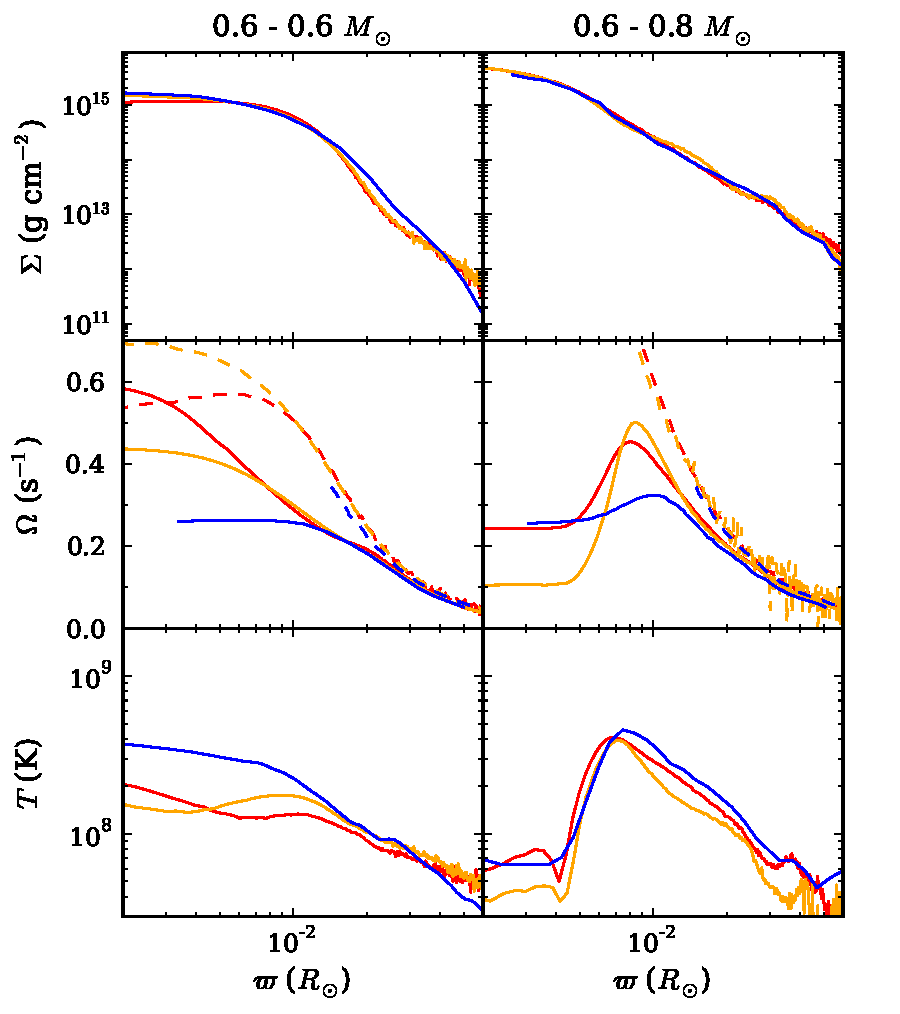
\includegraphics[angle=0,width=0.5\columnwidth]{chapter2_zhu+13/figures/compwithloreig.pdf}
\caption{Comparison of our results with those of \citetalias{loreig09}, for a 0.6 - 0.6\,\Msun\ (left) and a 0.6 - 0.8\,\Msun\ (right) merger.  Shown are surface density, remnant (solid) and Keplerian (dashed) angular frequency, and temperature, with profiles from \citetalias{loreig09} in blue, and our equivalent ones in red and orange.  Here, the former are for our default completion time of 6 initial orbital periods and the latter for their completion times (514 s or 10.9 orbital periods for the 0.6 - 0.6\,\Msun\ merger, and 164 s or 3.4 orbits for the 0.6 - 0.8\,\Msun\ merger).}
\label{fig:c2_compwithloreig}
\end{figure}

%The differences between our results and those of \citetalias{loreig09} are not because of our 2.5\% non-axisymmetry merger completion criterion - Fig. \ref{fig:compwithloreig} also shows curves from our simulations at \citeal{loreig09}'s stated completion times, and these curves look a more similar to our results than \citeal{loreig09}'s.  Our differences could be due to differences in the artificial viscosity implementation, as we use the variable $\alpha$ scheme while \citetalias{loreig09} uses a method based on Riemann solvers.  They could also be due to initial condition setup.  \citeal{loreig09}'s binaries do not start close enough to each other to immediately prompt Roche Lobe overflow; instead, an artificial radial acceleration is used to slowly bring the two stars in until one begins to transfer mass to the other.

\subsection{Comparison with Others}
\label{ssec:c2_compwithothers}

Simulations of WD mergers have also been presented by \citet{yoonpr07}, \citet{pakm+10,pakm+11,pakm+12}, \citet{dan+11,dan+12}, and \citet{rask+12}.  Unfortunately, comparison with those results is difficult, since, unlike \citeal{loreig09}, all these authors are sparse with quantitative details about their results.

%run Analyzer.py pt8pt9o.36000.ascii
%[massR,massM] = getmassr(gasr, gasmass, dR)
%[densoutputR_S, densoutputval_S] = getsphericaldensity(gasx, gasy, gasz, gasdens, dR)
%[TempoutputR_S, Tempoutputval_S] = gettemphelm(gasx, gasy, gasz, gastemp, gasdens, dR)
%plt.plot(massR*6.95508e9/1e9,massM/1.9891e33,'r-')
%plt.semilogy(densoutputR_S*6.95508e9/1e9,densoutputval_S)
%plt.semilogy(TempoutputR_S*6.95508e9/1e9,Tempoutputval_S)

An exception is the 0.81 - 0.9 {\Msun} merger simulated by \cite{dan+12}, shown in their Fig.~1.  While that simulation is for synchronized WDs, it is still particularly useful to compare with, since \citeauthor{dan+12} show results for both approximate and accurate initial conditions.  We find that their spherically enclosed mass profile is very similar to ours, with, e.g., $M=0.9\,\Msun$ at $4.5\times10^8\,$cm in both (though since spherically enclosed mass is a cumulative quantity, significant structural differences can remain hidden).  Our spherically averaged density profile looks most similar to the profile they found using approximate initial conditions.  Our central density, $1.9\times10^7\,\gcc$, is within $\sim\!10$\% of theirs, and the density profile remains similar up to $r \simeq 5 \times 10^8\,$cm ($\rho\simeq10^6\,\gcc$).  Beyond, their profile becomes shallower while ours continues to decline; at $r=10^9\,$cm, they find $\rho\simeq3\times10^5\,\gcc$, while we find $\rho\simeq10^5\,\gcc$.  This may be a consequence of the additional angular momentum associated with synchronized rotation.  With accurate initial conditions, a difference with our results is that the density profile becomes flat beyond $10^9\,$cm.  

Comparing temperature profiles, we roughly reproduce their spherically averaged one for approximate initial conditions, including the off-center peak -- their \Tmax\ is $\sim\!20\%$ lower (to be expected since their binary is synchronized; see Sec.~\ref{ssec:c2_synchronization}), but is also located at $4\times10^8\,$cm (or $M_r\simeq0.9\,\Msun$).  However, our central temperature ($2.2\times10^8$ K) is an order of magnitude higher than theirs ($2\times10^7$ K) and at $r\gtrsim10^9\,$cm our temperatures are systematically hotter, perhaps a result of the much larger dissipation expected for non-rotating WDs.  With accurate initial conditions they found an even narrower temperature peak than the one with approximate conditions, which thus deviates even more from our curve.  This trend is similar to what we see when increasing \azero\ (Sec.~\ref{ssec:c2_varyingazero}), so it seems likely we would reproduce their simulations more closely if we used the same initial conditions.

\subsection{The Importance of Accurate Initial Conditions}
%MHvK: I felt this could use its own subsection.

Many of the recent simulations \citep{dan+11,dan+12,rask+12} assume co-rotating WDs.  This assumption is numerically convenient, in that it is relatively straightforward to start the simulation in the physically correct state: since in the co-rotating frame there are no flow velocities, one can easily relax a simulated binary within an appropriate potential in the co-rotating frame, damping out any velocities resulting from an initial mismatch.  

As a result, it has been possible to study the onset of mass transfer in detail.  As first pointed out by \citet{dsou+06} from simulations using a grid code, the disruption of the donor is preceded by a rather long -- dozens of orbits -- phase of mass transfer.  Further simulations by \cite{dan+11,dan+12} showed that in this initial phase a significant fraction, $\sim10\%$ of the donor mass, is transferred.  As a result, e.g., the disk is substantially colder and more extended.  The remnant core seems more subtly affected, in that its appearance becomes ``more dissimilar'', reflecting that coalescence is between two WDs whose masses have become more disparate than they were initially.  As a consequence, e.g., even for similar-mass binaries, the hottest point of the merger is found to be well outside the center.  Indeed, \citet{rask+12} find that even for equal-mass binaries, the final outcome for more massive mergers is one where the core of one of the WDs is virtually undisturbed.

%(i.e. evolution following full disruption of the donor)

%MHvK: not sure if we should remove it, but in the end I felt it distracted from the discussion; I added just a short sentence in the section above
%If the primary differences between our simulations and those of \cite{dan+12} are an extended period of mass transfer and synchronization, we can use the results of Sec. \ref{ssec:varyingazero} and Sec. \ref{ssec:synchronization}.  We found above that synchronized mergers have colder cores and slightly narrower off-center temperature plateaus, and an extended period of mass transfer has a similar effect.  For equal mass mergers, synchronizing and an extended period of mass transfer also have the effect of slightly increasing the spherical density of material at larger distances from the remnant center.  This suggests that we would much more closely reproduce the results of \cite{dan+12} if we used synchronized, accurate ICs.

%Nevertheless, we can use these {\azero} tests as a poor proxy of what the effect might be.  They show a trend toward less mixing between the two WDs and more narrowly peaked off-center temperature and angular velocity curves with increasing {\azero}.  A larger {\azero} also results in the binary surviving for many more orbits before total disruption of the donor is achieved.  Moreover, since a small amount of mass transfer occurs during this period of time, perhaps enough mass is transferred to render an equal mass merger ``dissimilar-mass'' at coalescence.  It is therefore possible that increasing {\azero} for equal mass mergers would allow us to qualitatively reproduce the results of \cite{dan+11,dan+12} and \citet{rask+12}.

At present, it is not clear how important accurate initial conditions would be for asynchronous mergers.  Qualitatively, we expect the effects to be smaller than for synchronous mergers, for three reasons.  First, from the analytic study of \cite{lairs94}, in which tidal and rotational distortion are approximated by ellipsoids, co-rotating binaries always reach contact or Roche lobe overflow before becoming dynamically unstable, while irrotational binaries become dynamically unstable first.  While an exact treatment of the irrotational case found that, in fact, Roche contact preceded dynamical instability \citep{uryue98}, it suggests that WDs in irrotational binaries will disrupt much sooner.  Second, the simulations of \citeal{loreig09} use initial conditions that should be quite close to correct, yet their WDs disrupt quickly (see Sec. \ref{ssec:c2_compwithloreig}).  Third, the two components are counterrotating in the rotating frame.  Hence, any mass transferred will hit the accretor with a larger relative velocity than would be the case for co-rotating WDs.  Indeed, in the limit of equal-mass WDs, very little would happen for co-rotating WDs when one reaches contact, while a strong shock would be expected for the irrotational case.  In general, one expects part of the shocked material to enter a high-entropy halo around the accretor.  For co-rotating WDs, \cite{dan+11} found that this halo helps remove angular momentum from the orbit, leading to a shorter start-up phase.  For the irrotational case, given the stronger expected shocks, the start-up phase would likely be reduced even further.  On the other hand, we saw in Sec. \ref{ssec:c2_varyingazero} that remnant properties are sensitive to changes in angular momentum content through changes in \azero.  Simulating more realistically the onset of mass transfer through accurate initial conditions will likely change \azero.

Ideally, one would still simulate the initial mass transfer phase accurately.  Unfortunately, even though the equilibrium solution is known \citep{uryue98}, it is not straightforward to set up the initial binary properly, since it is difficult to relax to a state that includes substantial fluid motion, and to slowly evolve such a state to contact, while ensuring viscosity remains low enough that there is no artificial tidal dissipation.  Such dissipation is seen in our tests with varying initial distance {\azero} in Sec.~\ref{ssec:c2_varyingazero} (and may affect the simulations of \citeal{loreig09} as well).  Prior to coalescence, strong dissipation of tidal bulges heats the outer envelope of the donor (both stars for similar-mass mergers), and spin-orbit coupling due to both tides and the direct-impact accretion stream result in both donor and accretor becoming 25 - 50\% synchronized by coalescence.

Since it significantly affects the merger and merger outcome, whether or not tidal dissipation causes real CO WD binaries to synchronize before the merger remains a major source of uncertainty.  For the radiative stellar envelopes appropriate for WDs, tidal dissipation is expected to be inefficient, with a timescale $10^{12}$ to $10^{15}$ yrs, suggesting that WDs do not synchronize (\citealt{marsns04}, and references therein).  However, coupling of the tides to pulsations may dramatically increase dissipation \citep{fulll12}.  Fortunately, it may be possible to determine the rate of synchronization observationally.  For instance, \citet{piro11} suggested that tidal dissipation is responsible for the relatively high temperature of the primary WD in the 13-minute eclipsing binary SDSS J065133.33+284423.3, predicting that it would be about halfway to being synchronized.  This could be tested by either measuring the rotational broadening of the narrow cores of the hydrogen lines, or looking for velocity deviations through the transit of the more massive secondary.

%For discussion/outlook (mostly from my proposal; edit at will)

%A major uncertainty in all simulations is whether or not the white dwarfs co-rotate before the merger.  Theoretically, the rate of dissipation is difficult to estimate.  
%Probably not needed
% For convective envelopes, theory matches observations for giants, where convective turn-over times are slow compared to the orbit, but not for main-sequence stars, where they are fast, and hence we still do not understand, e.g., how main-sequence binaries can be
% circularized up to $\sim\!10\,$d periods (for a review, Zahn 2008).

%citation{dan+11}{2011ApJ...737...89D}
%citation{dan+12}{2012arXiv1201.2406D}
%citation{dsou+06}{2006ApJ...643..381D}
%citation{fryed08}{2008ASPC..391..335F}
%citation{fulll12}{2012MNRAS.tmp.2242F}
%citation{marsns04}{2004MNRAS.350..113M}
%citation{pakm+10}{2010Natur.463...61P}
%citation{pakm+11}{2011A&A...528A.117P}
%citation{pakm+12}{2012arXiv1201.5123P}
%citation{piro11}{2011ApJ...740L..53P}
%citation{rask+12}{2012ApJ...746...62R}
%citation{uryue98}{1998ApJS..118..563U}
%citation{yoonpr07}{2007MNRAS.380..933Y}
